\section{Experiments}

\subsection{MONK's results}

\subsubsection{Architecture and hyperparameters}
We have used a fully connected NN with layers of size 17-15-2, with a $\tanh$ activation in the hidden layer, and a \texttt{softmax} activation for the output layer.

We choose \texttt{categorical\_crossentropy} as the loss function, i.e. if the output of the NN is $y=(y_1,y_2)$ and the label is $\hat y=(\hat y_1,\hat y_2)$, then $$L(y,\hat y)=-\hat y_1\log y_1-\hat y_2\log y_2$$

We use mini-batch gradient descent with $\texttt{batch\_size}=32$ and momentum with parameter $\beta$.

We also use L2 regularization with parameter $\lambda$.

\begin{figure}
    \caption{Performance results on MONK dataset}
    \label{fig:hyper}
    \begin{tabular}{|l|c|c|c|c|c|}
        \hline 
        Task & $\eta$ & $\lambda$ & $\beta$ & Loss (train/valid) & Accuracy (train/test) \\ \hline
        MONK 1 & 0.1 & 0.003 & 0.8 & 0.0466/0.0552  & 100\%/100\% \\ \hline
        MONK 2 & 0.1 & 0.003 & 0.8 & 0.0531/0.0896 & 100\%/100\% \\ \hline
        MONK 3 (reg) & 0.01 & 0.02 & 0.9 & 0.2116/0.4599 & 94.2\%/97.2\% \\ \hline
        MONK 3 (non reg) & 0.1 & 0.0001 & 0.9 & 0.0052/0.7687 & 100\%/93.9\% \\ \hline
    \end{tabular}
\end{figure}

Our choice of hyperparameters is shown in \cref{fig:hyper}, along with the performance.


\subsubsection{Learning curves}

Now we show the learning curves of the three MONK tasks, plotting loss and accuracy over the training set and the validation set.

\begin{figure}
    
    \centering
    \subfloat[MONK 1]{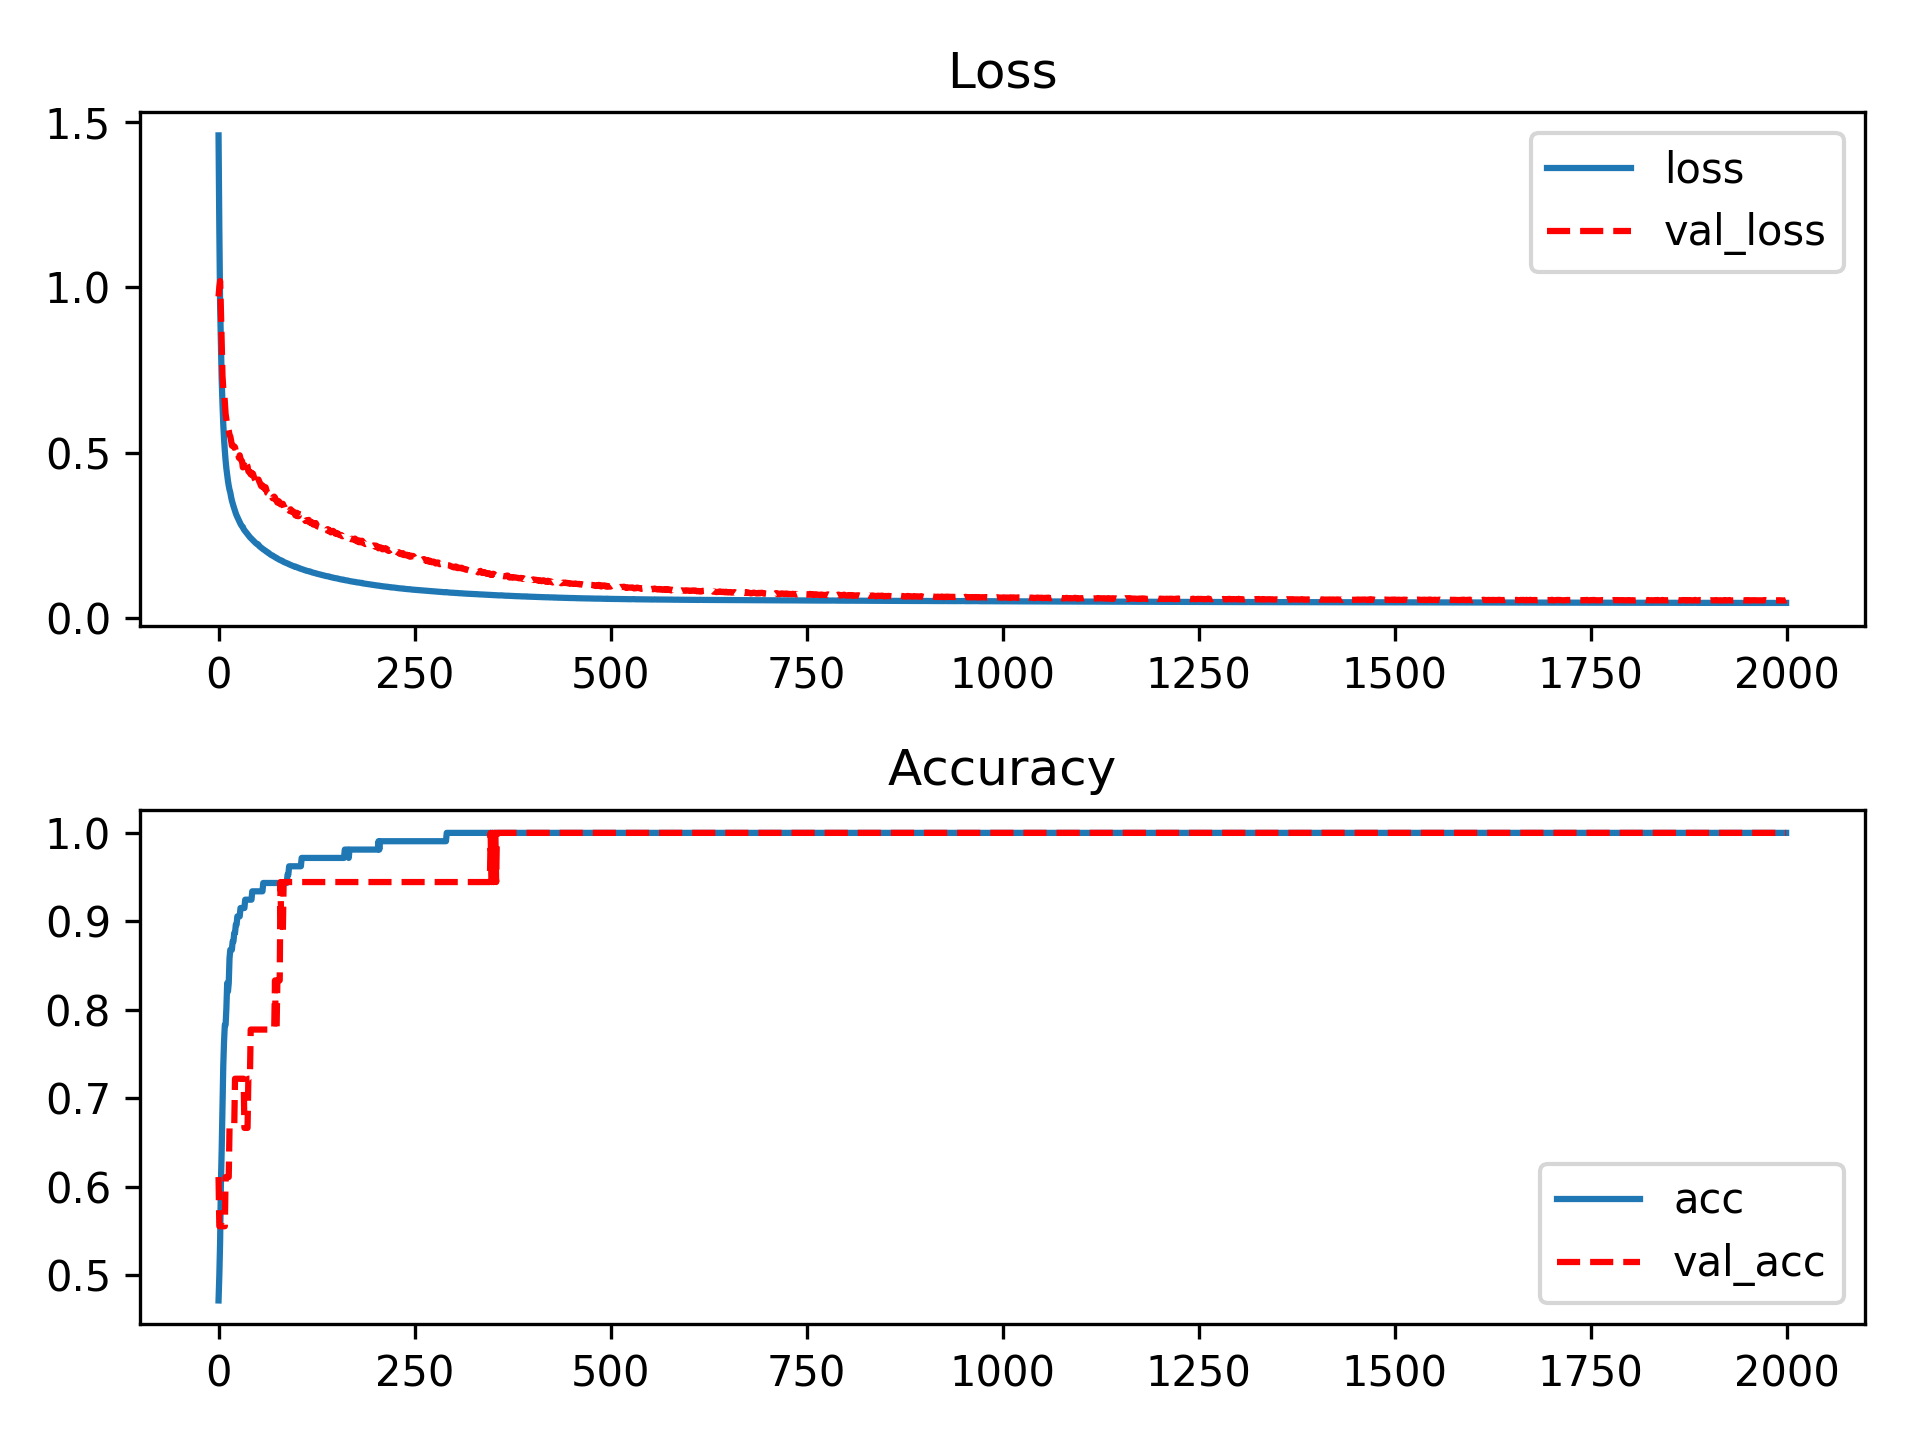
\includegraphics[width=0.5\textwidth]{monks1}}
    \subfloat[MONK 2]{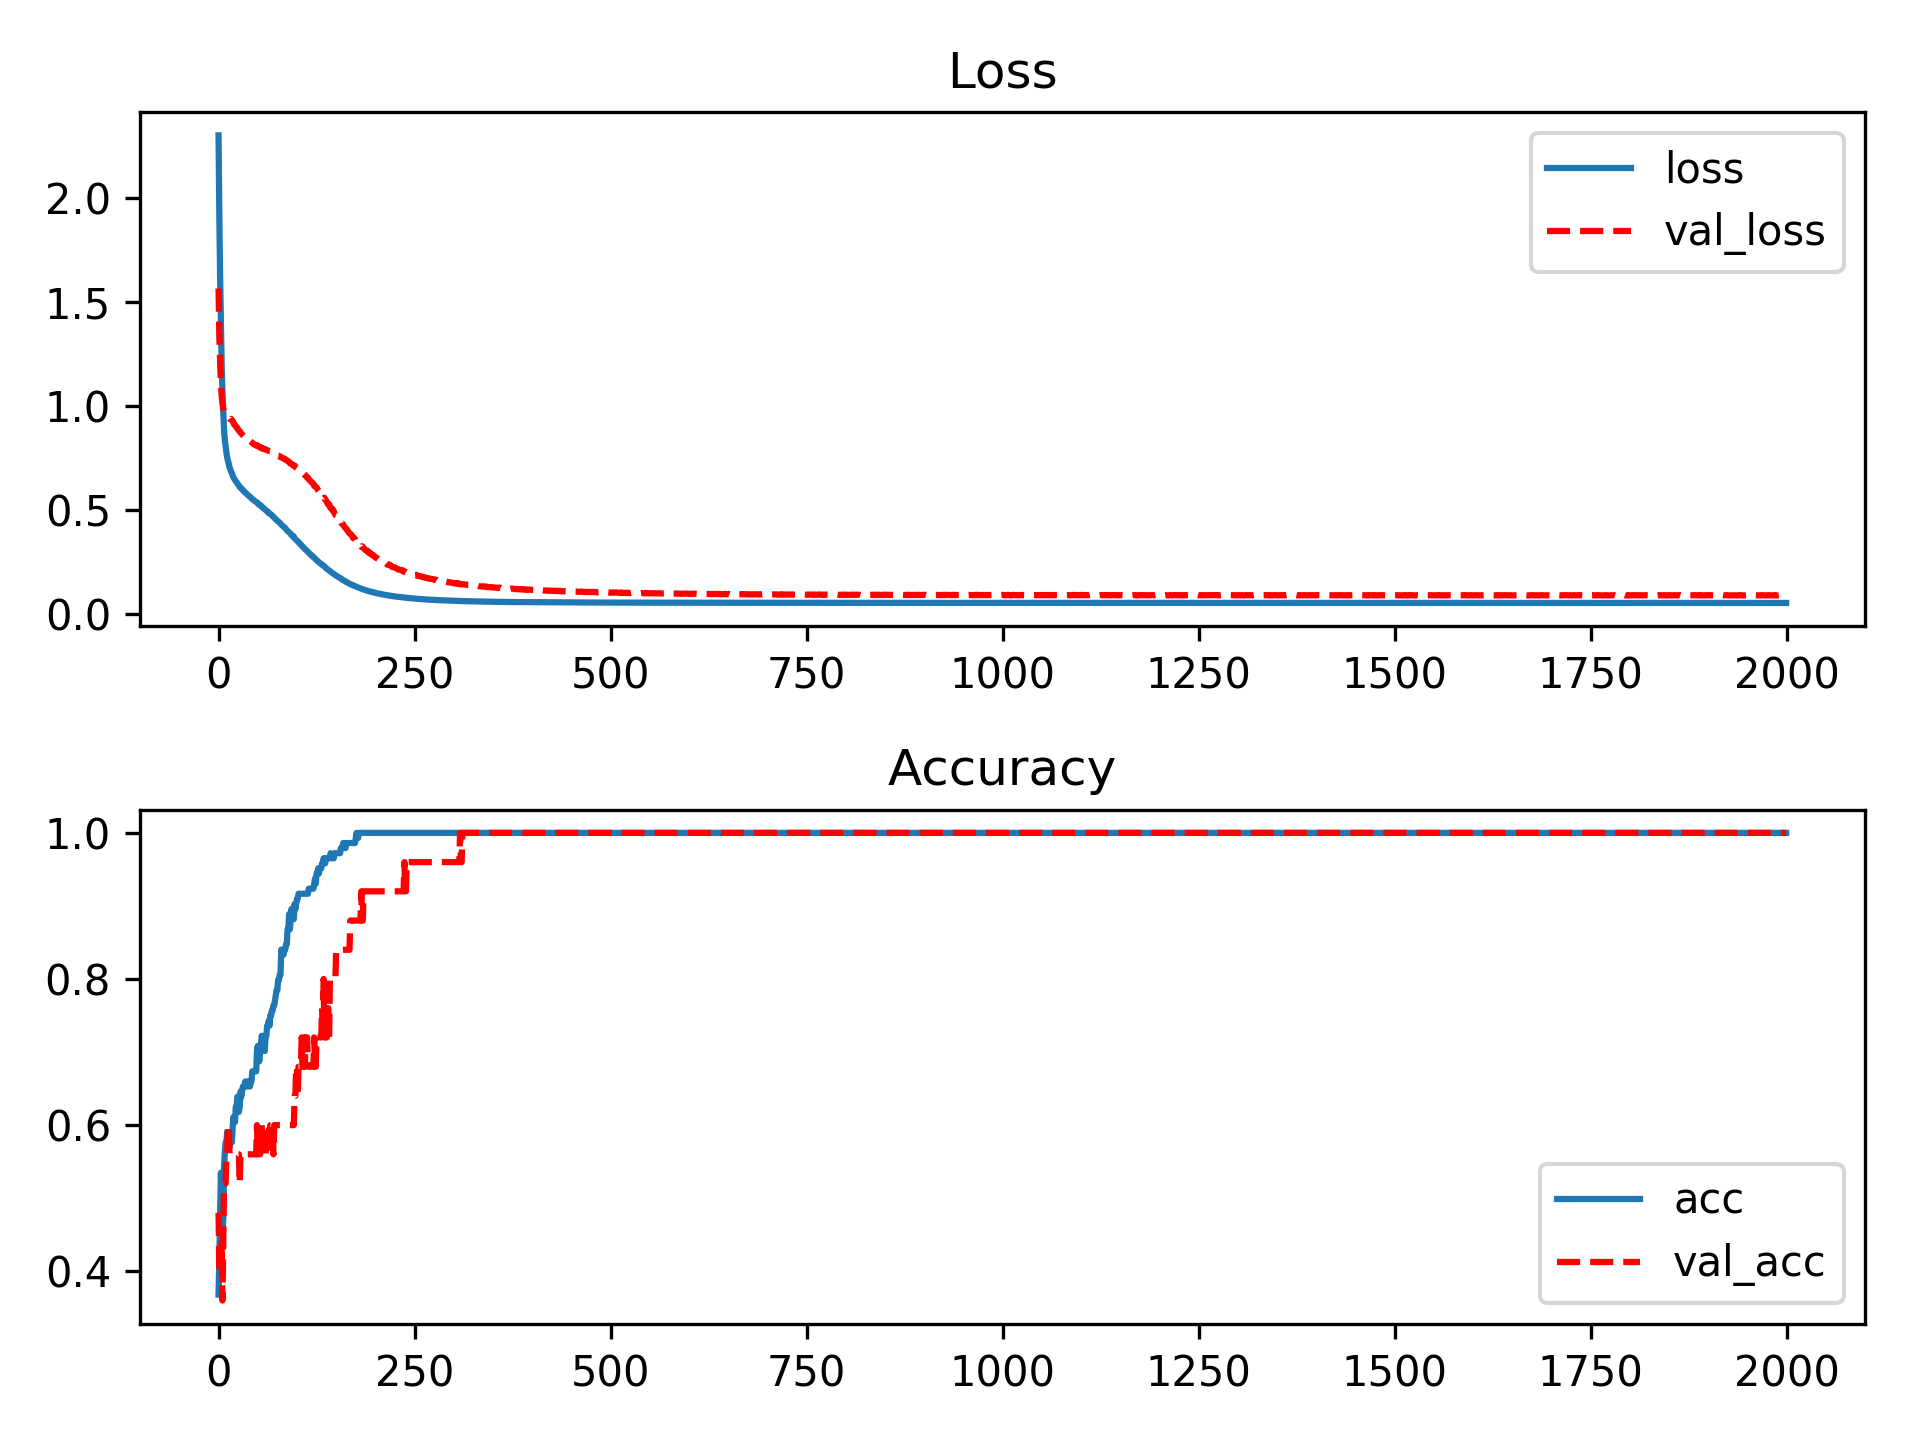
\includegraphics[width=0.5\textwidth]{monks2}}
    \caption{Learning curves on MONK 1 \& 2}
    \label{fig:monk12}

\end{figure}



\begin{figure}
    \centering
    \subfloat[regularized\label{fig:monk3}]{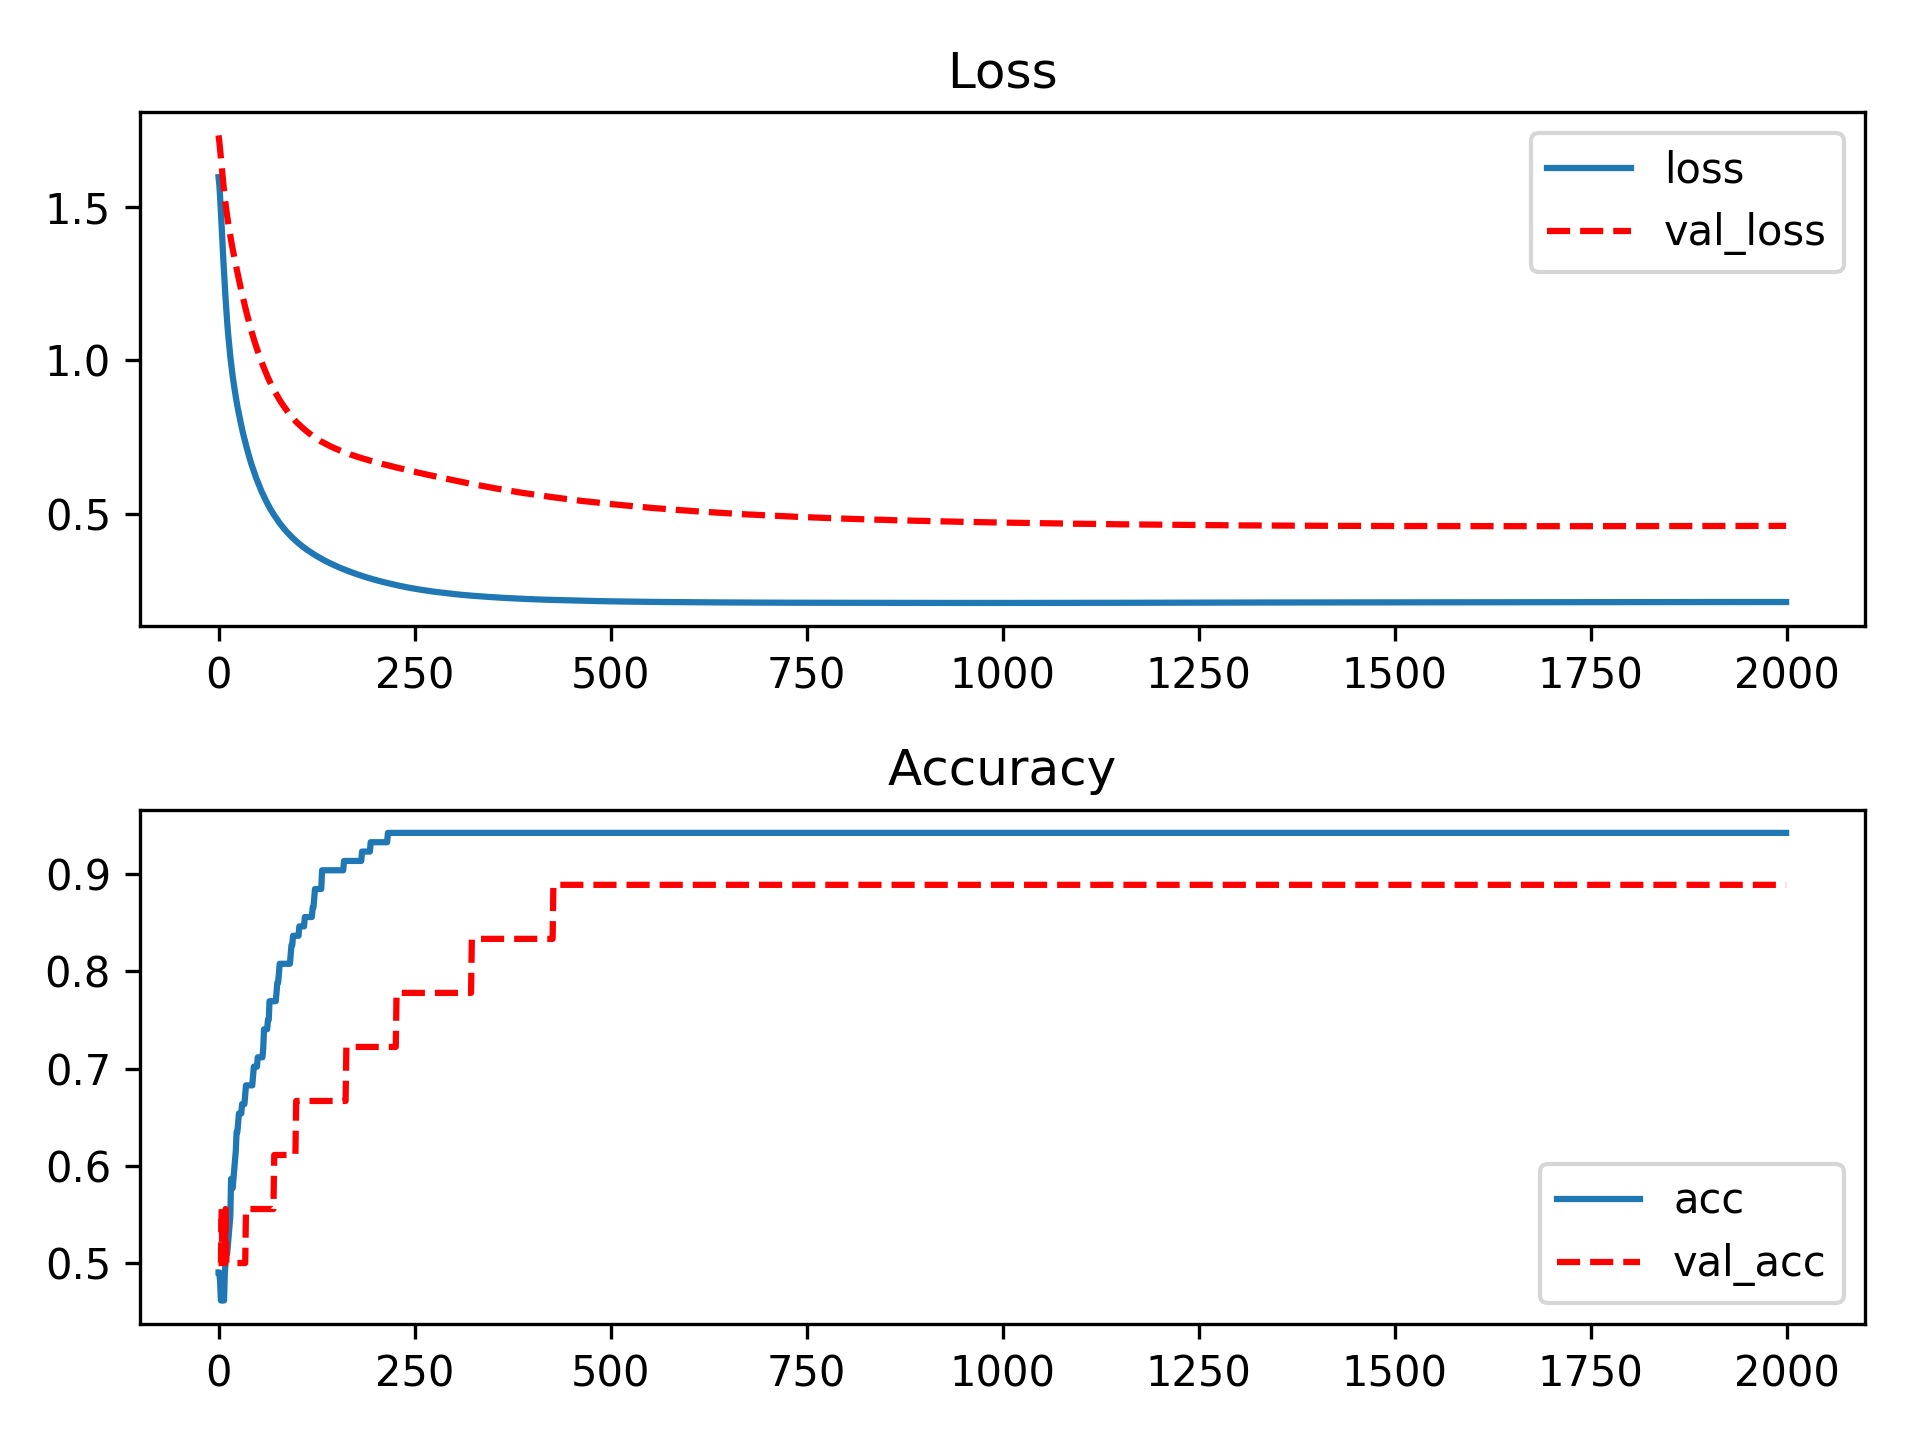
\includegraphics[width=0.5\textwidth]{monks3}}
    \subfloat[not regularized\label{fig:monk3-nr}]{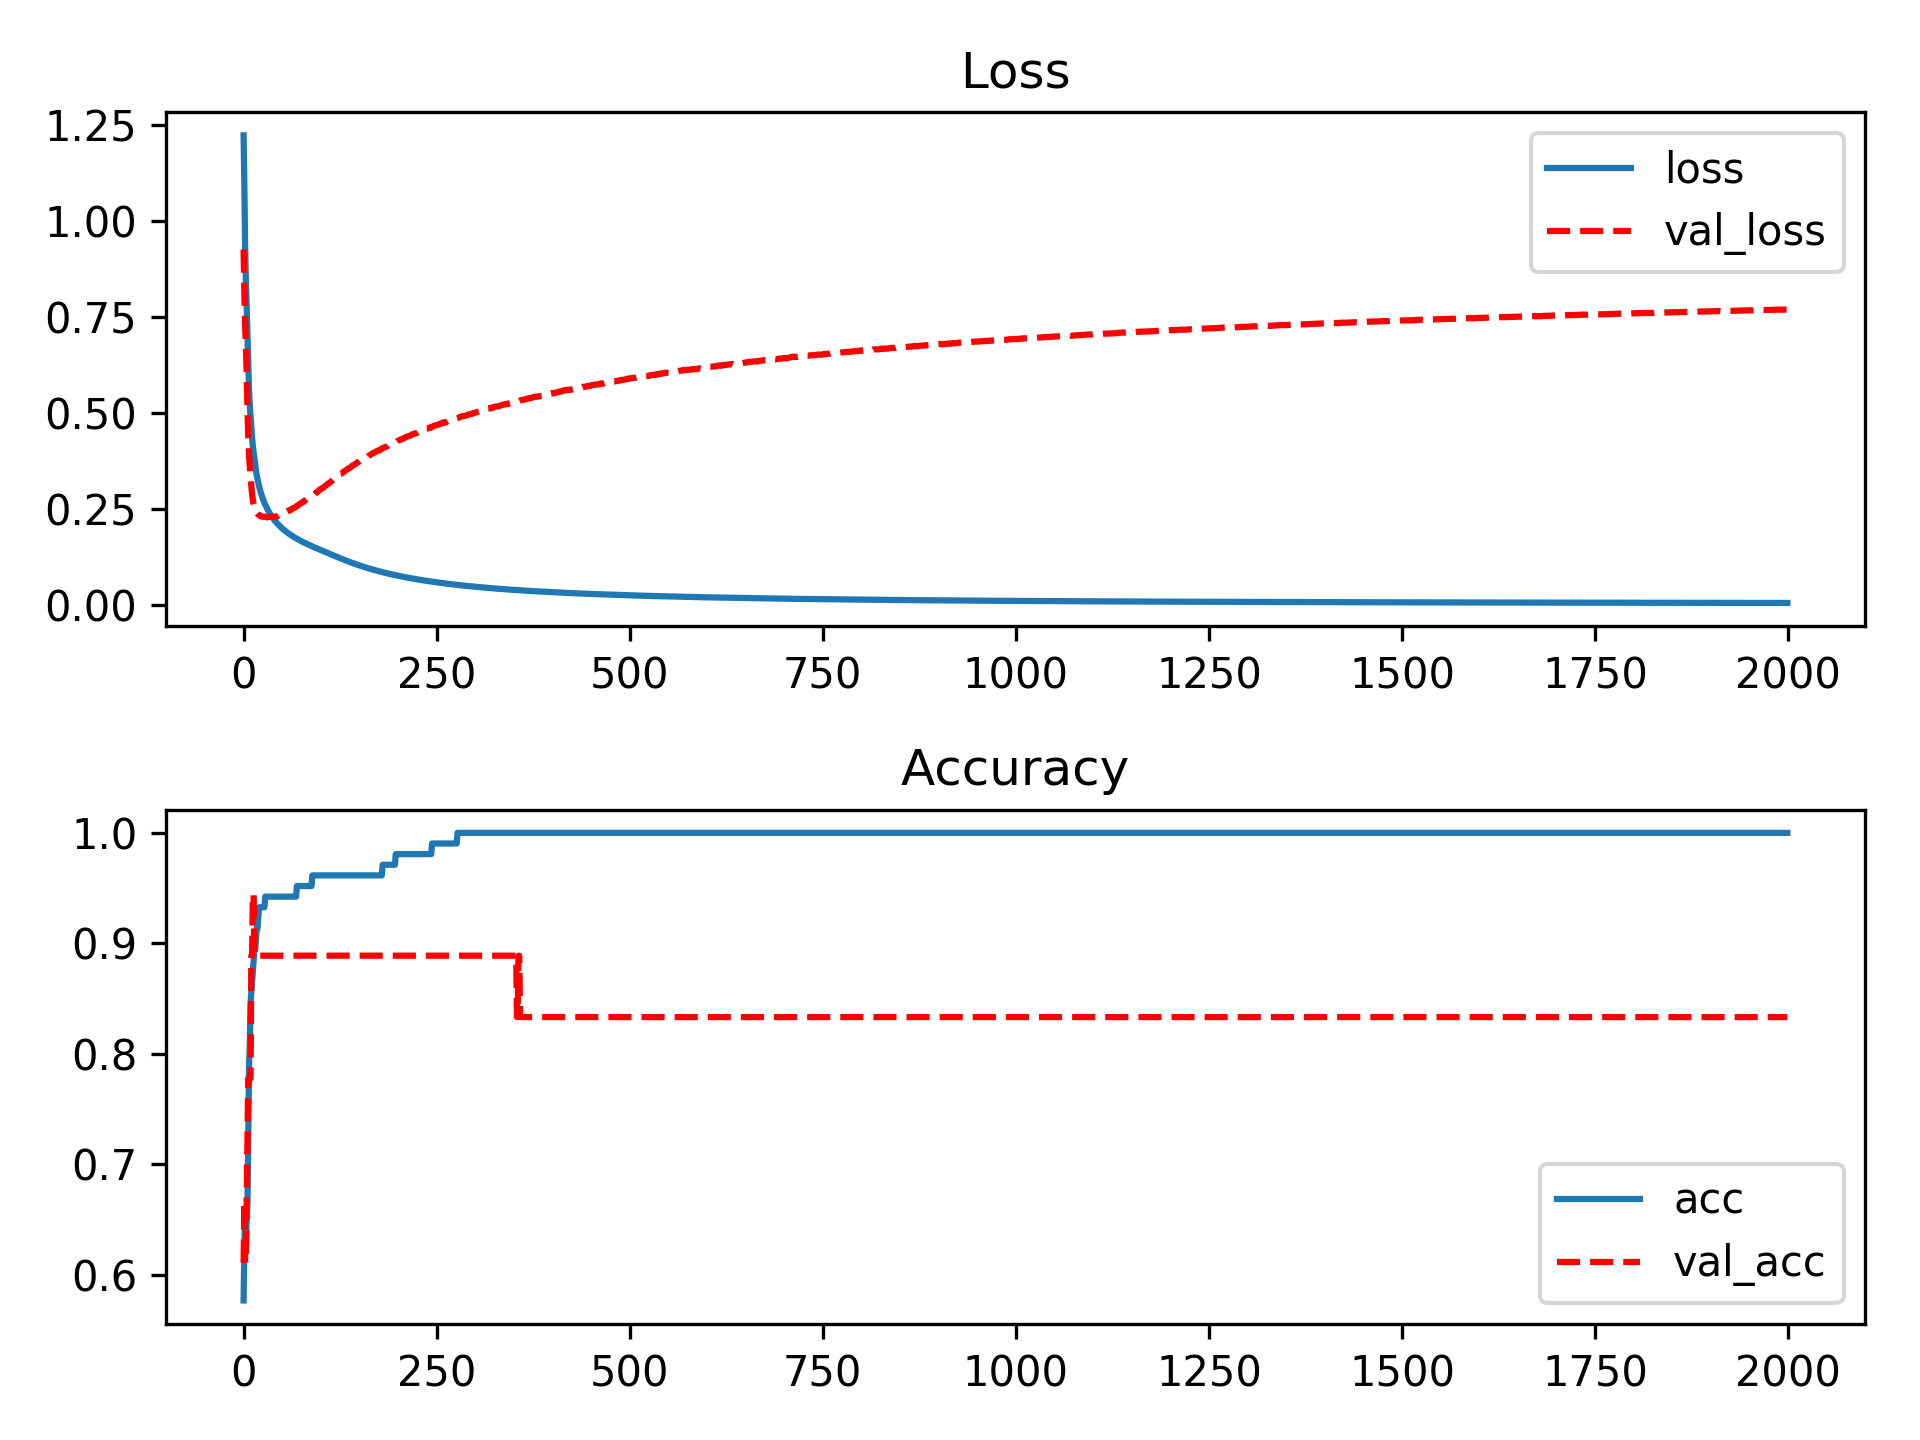
\includegraphics[width=0.5\textwidth]{monks3-nr}}
    \caption{Learning curves for MONK 3}
\end{figure}


We notice that the training loss of MONK 3 (\cref{fig:monk3}) is quite high: this is because the training set has noise, and we are keeping a quite strong regularization.
If instead we remove the regularization, then it overfits as shown in \cref{fig:monk3-nr}


\clearpage

\subsection{CUP results}

The first thing we did was to take 100 random datapoints from the training set and put them in a separate file for internal testing. So we had 916 datapoints for the actual training and validation.

For every training instance we randomly split the internal training set at random for 75\% actaul training and 25\% validation.

\subsubsection{Preliminary trials}

We first tried to see if we needed a deep NN, but increasing the number of layers didn't bring significant improvements.

Then we choose to use MEE as the loss function instead of MSE, because it's the actual metric we want to mimnimize.

So we wanted a model with layers 10-H-2 for some $H\in\{ 10, 20, 50 \}$, and an activation function in the hidden layer among \texttt{tanh}, \texttt{sigmoid}, \texttt{reLU}.

Then we had also to tune the hyperparameters $\eta,\lambda,\beta$ so we did a grid search on these 5 parameters, distributing the load to many machines.

\subsubsection{Grid search}

For each choice of activation function and number of hidden neurons $H$ we had a different machine run a grid search among these values:
\begin{itemize}
    \item $\eta\in\{ 0.1, 0.05, 0.01, 0.005, 0.001 \}$
    \item $\lambda\in\{ 0.005, 0.001, 0.0005, 0.0001 \}$
    \item $\beta\in\{ 0, 0.95 \}$
\end{itemize}

Our best results were with the \texttt{sigmoid} activation and $H=20$, on which we had the results shown in \cref{fig:gridsearch}.

\begin{figure}
    \centering
    \begin{tabular}{|c||c|c|c|c|c|}
            \hline
              $\lambda \backslash \eta$ & $0.1$ & $0.05$ & $0.01$ & $0.005$ & $0.001$\\ \hline\hline
             $0.005$ & 1.461 & 1.493 & 1.465 & 1.461 & 1.728 \\ \hline
             $0.001$ & 1.177 & 1.226 & 1.276 & 1.349 & 1.699 \\ \hline
             $0.0005$ & 1.193 & 1.175 & 1.249 & 1.317 & 1.668 \\ \hline
             $0.0001$ & 1.220 & 1.224 & 1.238 & 1.306 & 1.668 \\ \hline
    \end{tabular}
    \caption{Values of MEE for $H=20$, \texttt{sigmoid} and $\beta=0$}
    \label{fig:gridsearch}
\end{figure}

We run this grid search on multiple nodes in a single night: for each choice of hyperparameters we run the training for 2000 epochs for 10 trials, and then averaged the MEE score on the validation set.

\subsubsection{Chosen models}


\begin{figure}
    \centering
    \subfloat[Type A\label{fig:typeA}]{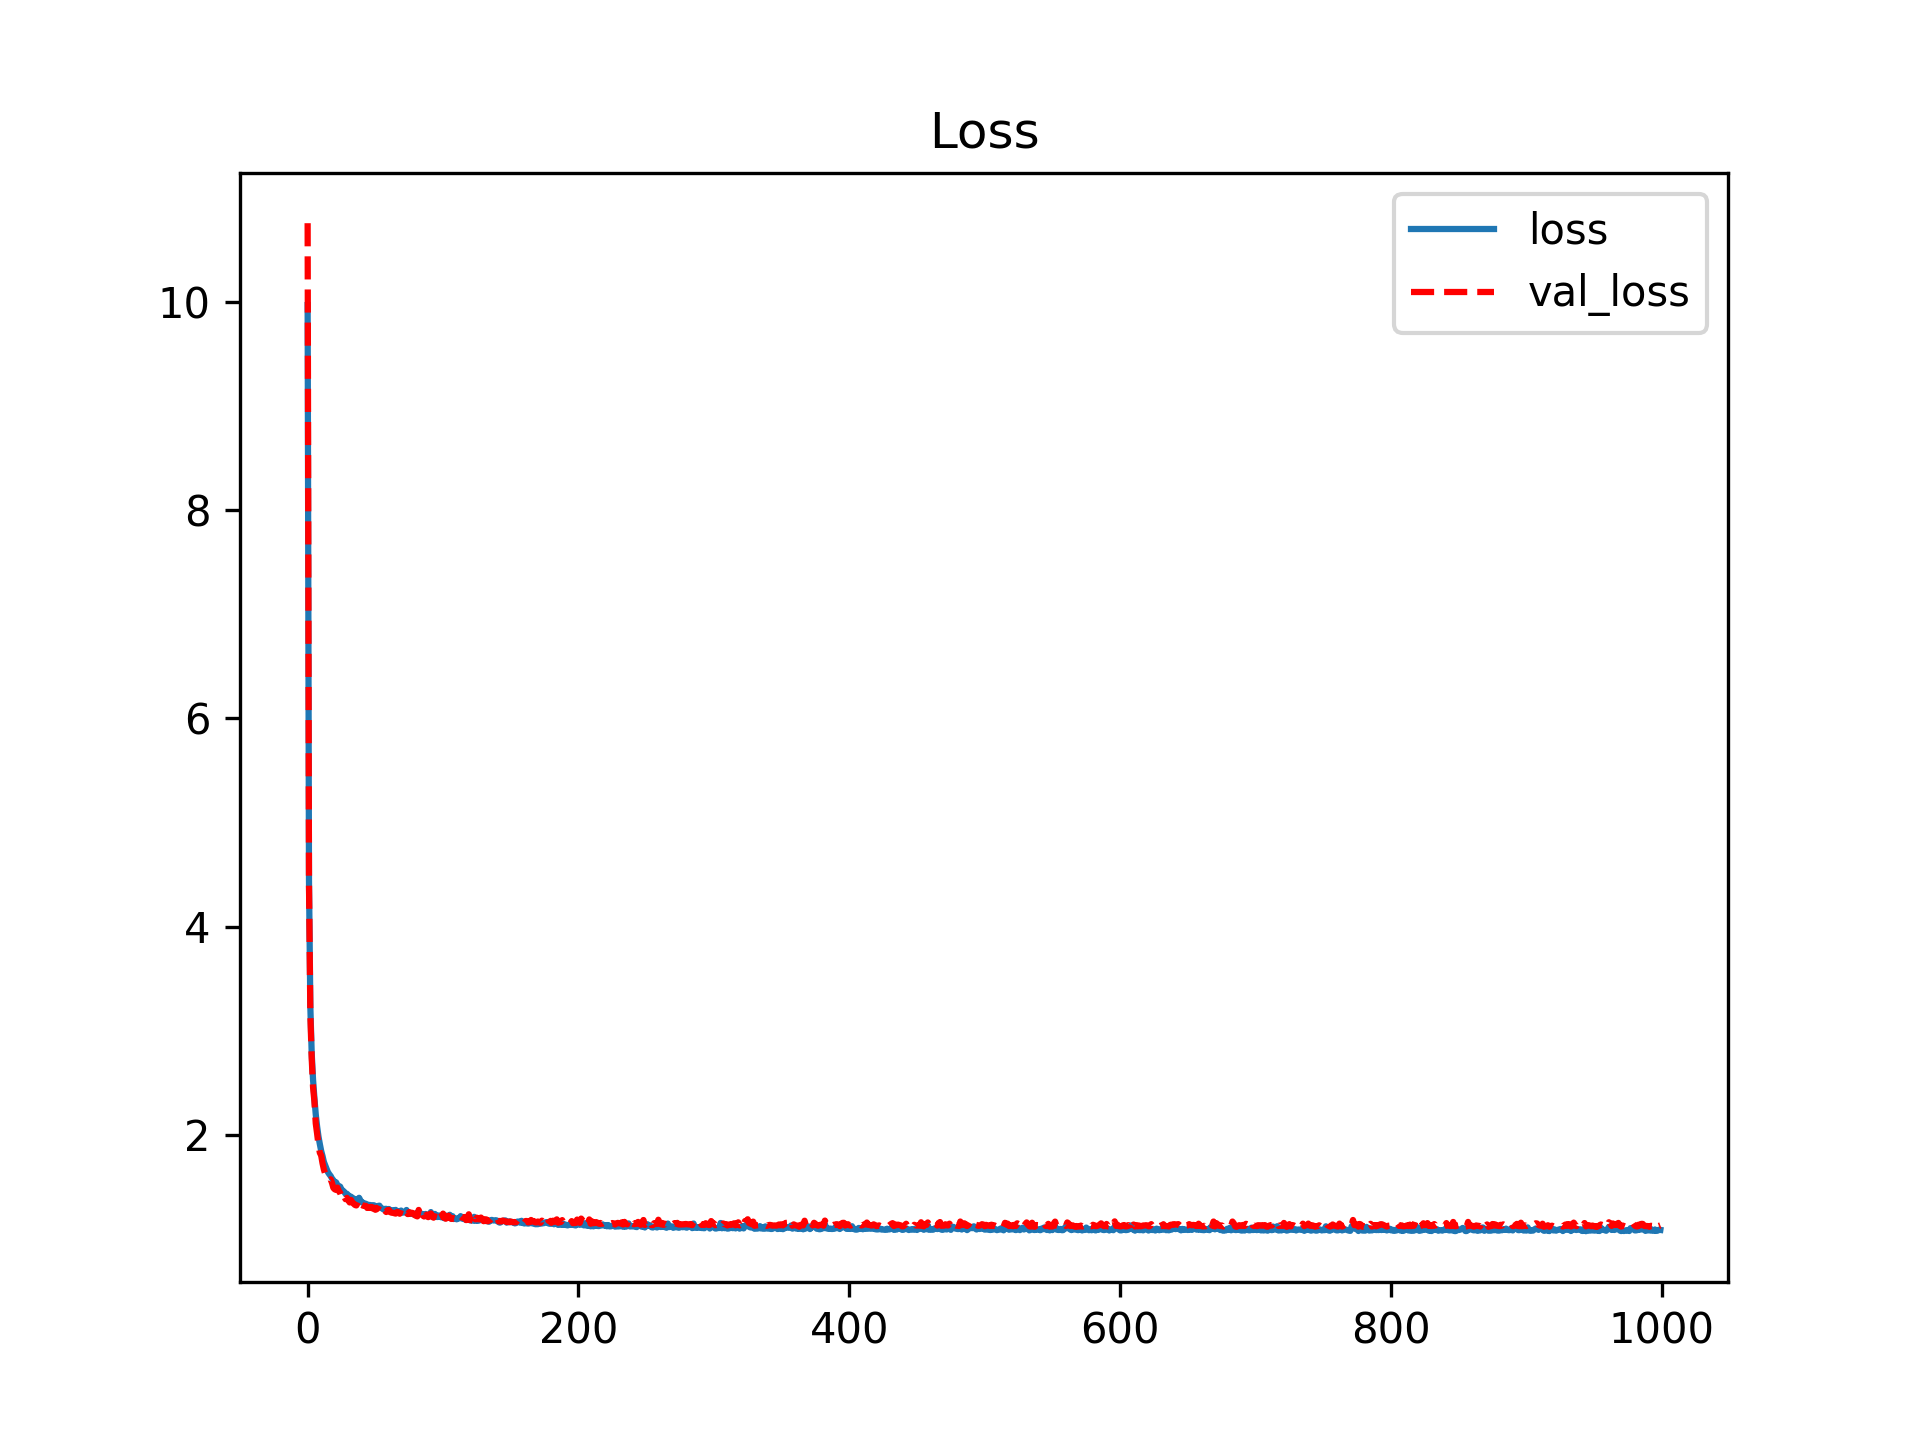
\includegraphics[width=0.55\textwidth]{cup10_one}}
    \subfloat[Type B\label{fig:typeB}]{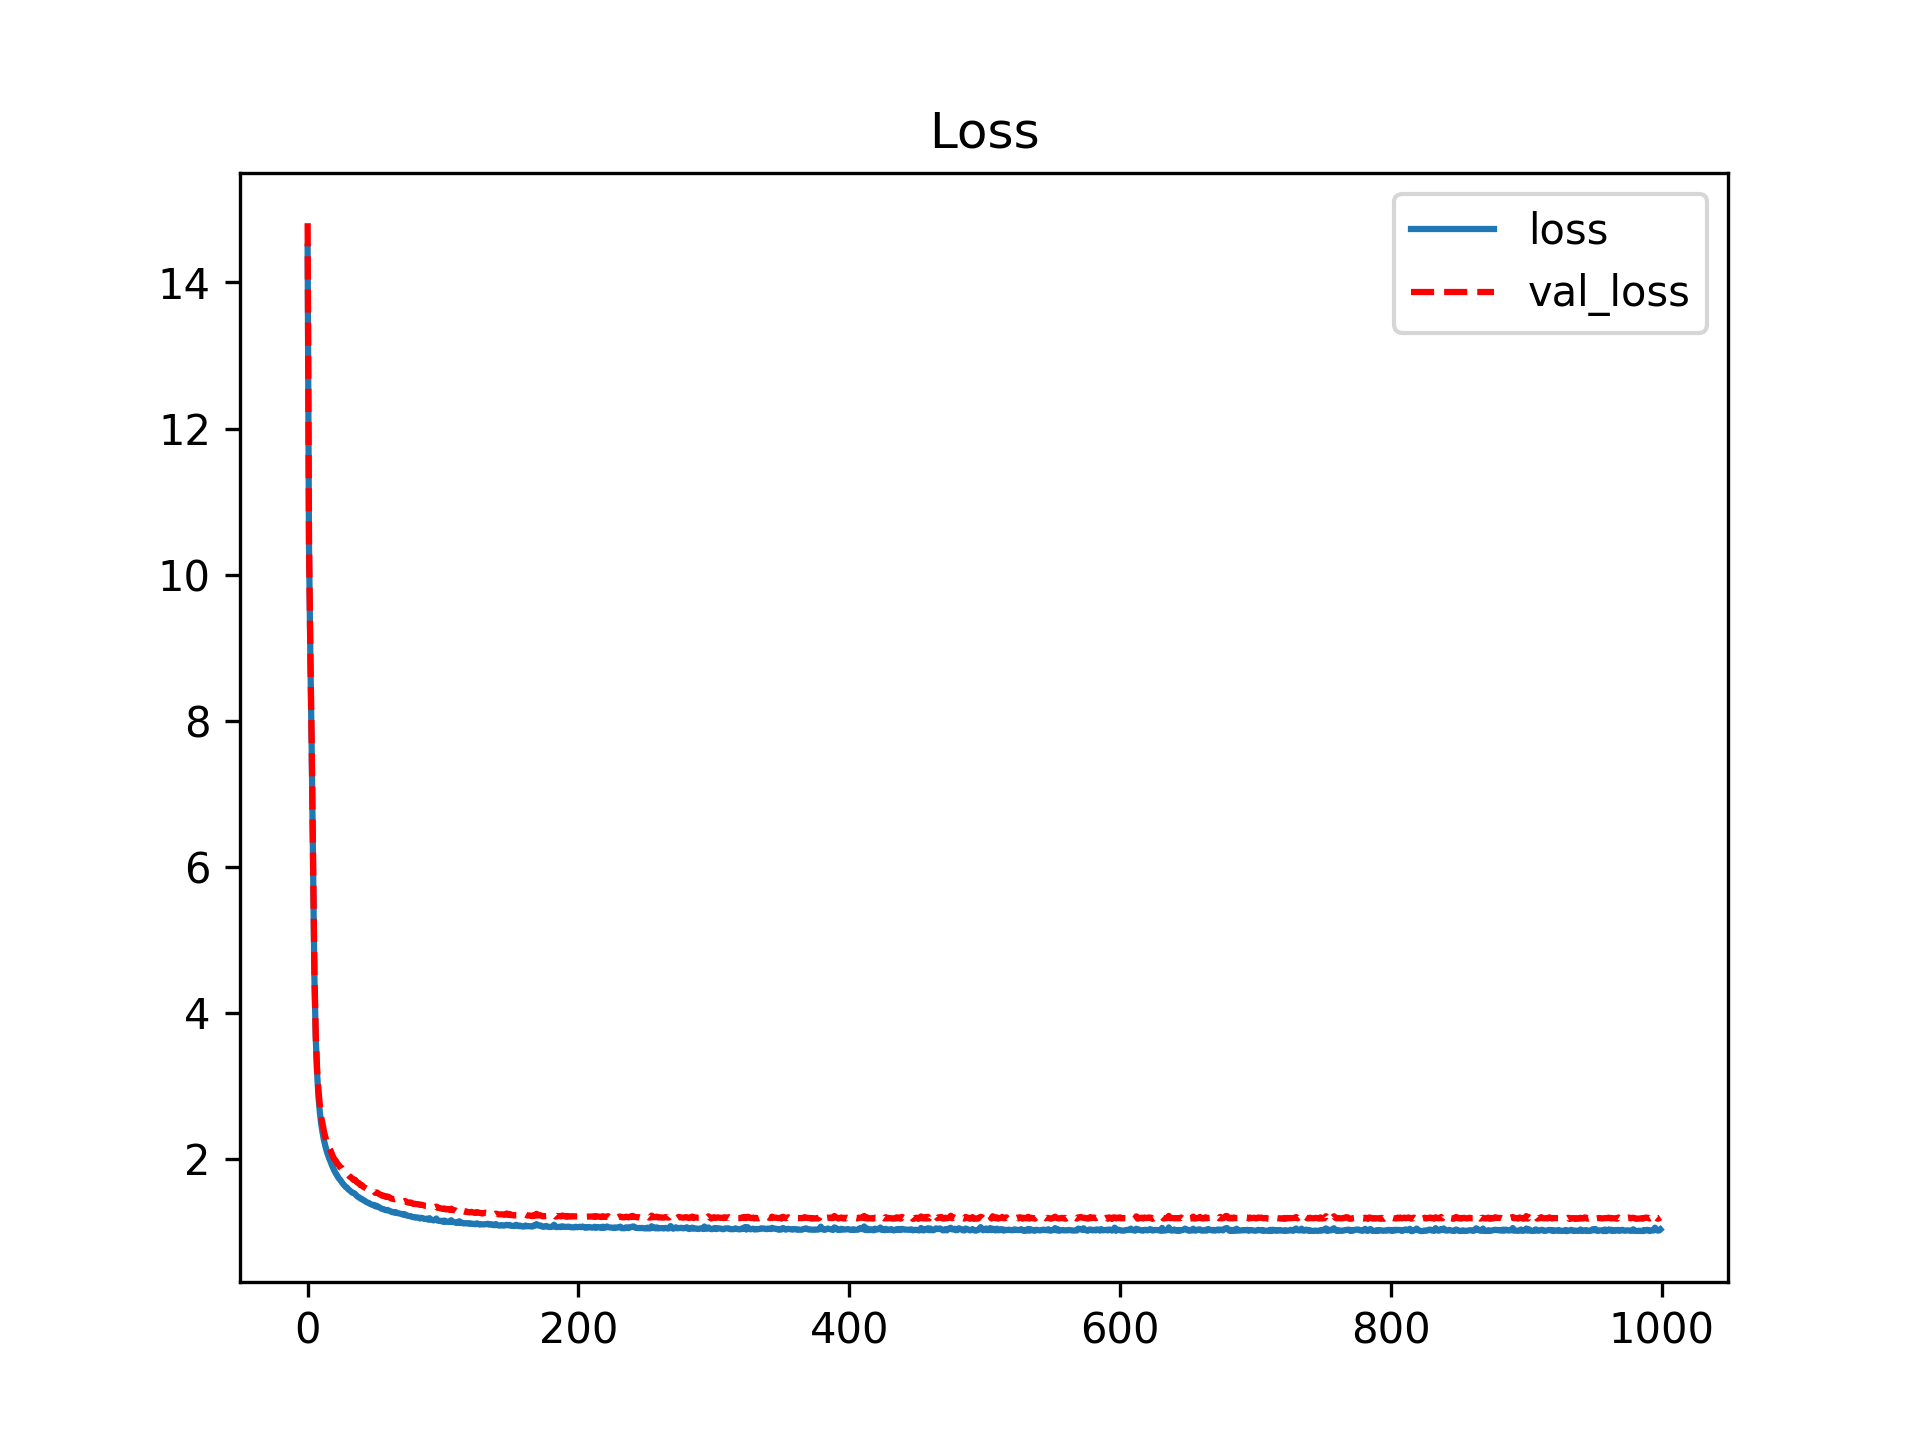
\includegraphics[width=0.55\textwidth]{cup55}}
    \caption{Learning curves for CUP networks}
\end{figure}


So our fist model had a topology of 10-20-2 with \texttt{sigmoid} activation, and we train it for 2000 epochs with $\eta=0.1,\lambda=0.001,\beta=0$. Let's call this \emph{network of type A}.

We achieved an average MEE of $1.119$ on our blind test, taken as an average of 10 different trainings of type A networks (to avoid the bias due to the random weight initialization). We can see the learning curve of one of them in \cref{fig:typeA}.

Then we tried an \emph{ensembling} approach: we trained 20 networks of type A and the output of our model would be the average of the outputs of the 10 best trained networks.

In this way we achieved a MEE error on the internal test set of $1.085$.

\bigskip
Our last model uses input preprocessing, and we use a different network architecture, say \emph{type B}.

The type B has a topology of 55-20-2, and is trained with $\eta=0.05,\lambda=0.005,\beta=0.9$.

The 55 inputs are calculated as follows from the dataset: if the original input is $(x_1,\dots,x_{10})$, our calculated new vector is $(x_1,\dots,x_{10},x_1\cdot x_2,\dots,x_9\cdot x_{10})$; we are thus appending the products of the input variables.

Then we take an ensembling approach and train 20 networks of type B, and we calculate the output by averaging the best 15 of them.

This ensemble of type B models achieve a MEE of $1.050$ on the internal test set.


\begin{figure}
    \centering
    \begin{tabular}{|l|l|l|}
        \hline
        id & Train MEE & Valid MEE \\ \hline
        3 & 1.030 & 1.129 \\ \hline
        5 & 0.968 & 1.250 \\ \hline
        8 & 1.038 & 1.081 \\ \hline
        15 & 1.011 & 1.148 \\ \hline
        20 & 0.987 & 1.327 \\ \hline
    \end{tabular}
    \caption{MEE of some of the ensembled type B networks}
    \label{fig:cup55-table}
\end{figure}


The learning curve of one instance of model B can be seen in the \cref{fig:typeB}. Values of training and validation MEE of some of the 20 models are in \cref{fig:cup55-table}.




%%% Local Variables:
%%% mode: latex
%%% TeX-master: "report"
%%% End:
